\section{El mecanismo de atención}
\label{sec:mecanismo_atencion}

Las secciones anteriores identificaron la limitación central de los modelos
clásicos: ninguno dispone de un mecanismo que permita que cada elemento de
una secuencia acceda, de forma dinámica y dependiente del contenido, a la
información de cualquier otro elemento. Esta sección presenta la solución
que los Transformers proponen: el \textit{mecanismo de atención}.

%------------------------------------------------------------
\subsection{Intuición: ¿qué significa ``prestar atención''?}
\label{subsec:atencion_intuicion}

La idea central es sencilla. Cuando un ser humano lee la oración
\textit{``El gato comió el ratón''} y quiere entender el verbo
\textit{comió}, no lo procesa en aislamiento: busca activamente quién
realiza la acción (sujeto: \textit{gato}) y sobre qué recae (objeto:
\textit{ratón}). Esta capacidad de enfocarse selectivamente en las partes
relevantes del contexto es exactamente lo que el mecanismo de atención
implementa de forma computacional.

Formalmente, para cada token de la secuencia, la atención calcula un
\textit{peso} $\alpha_{ij}$ que indica cuánta relevancia tiene el token $j$
para representar al token $i$. La representación final del token $i$ es
entonces una \textit{suma ponderada} de las representaciones de todos los
demás tokens:

\begin{equation}
    \bm{z}_i = \sum_{j=1}^{n} \alpha_{ij}\, \bm{v}_j
    \qquad \text{con} \quad \alpha_{ij} \geq 0, \quad \sum_j \alpha_{ij} = 1
\end{equation}

% ============================================================
% fig_atencion_intuicion.tex — Intuición del mecanismo de atención
% Uso: % ============================================================
% fig_atencion_intuicion.tex — Intuición del mecanismo de atención
% Uso: % ============================================================
% fig_atencion_intuicion.tex — Intuición del mecanismo de atención
% Uso: \input{figures/fig_atencion_intuicion}
% ============================================================
\begin{figure}[H]
\centering
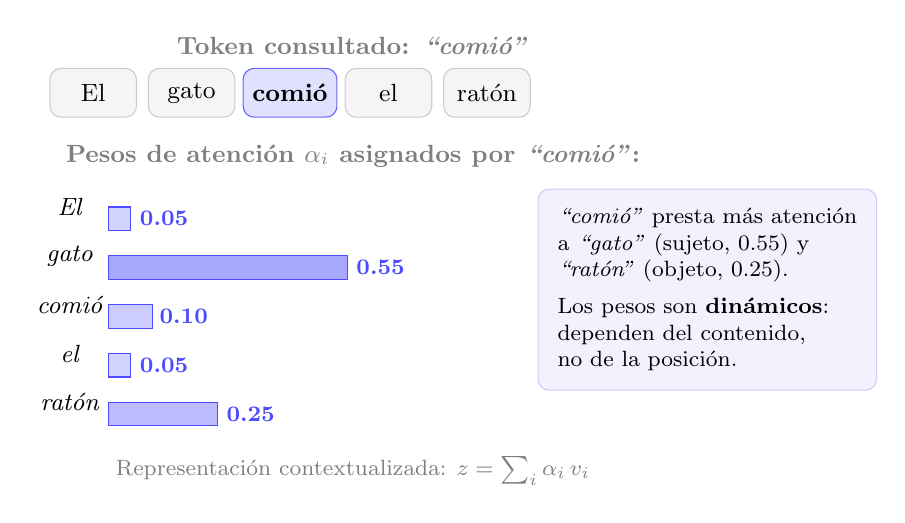
\begin{tikzpicture}[
    word/.style={draw=gray!40, rounded corners, fill=gray!8,
                 minimum width=1.1cm, minimum height=0.62cm, font=\small},
    focus/.style={draw=blue!60, rounded corners, fill=blue!12,
                  minimum width=1.1cm, minimum height=0.62cm,
                  font=\small\bfseries},
    weight/.style={font=\footnotesize\bfseries},
    bar/.style={fill=blue!50, draw=blue!70}
]

\node[font=\small\bfseries, gray] at (3.3, 5.6)
    {Token consultado: \textit{``comi\'o''}};

\node[word]  at (0*1.25, 5.0) {El};
\node[word]  at (1*1.25, 5.0) {gato};
\node[focus] at (2*1.25, 5.0) {comi\'o};
\node[word]  at (3*1.25, 5.0) {el};
\node[word]  at (4*1.25, 5.0) {rat\'on};

\node[font=\small\bfseries, gray] at (3.3, 4.2)
    {Pesos de atenci\'on $\alpha_i$ asignados por \textit{``comi\'o''}:};

\node[font=\small\itshape] at (-0.3, 3.55) {El};
\fill[bar, fill opacity=0.35] (0.2, 3.25) rectangle (0.475, 3.55);
\node[weight, blue!70] at (0.9, 3.40) {0.05};

\node[font=\small\itshape] at (-0.3, 2.93) {gato};
\fill[bar, fill opacity=0.685] (0.2, 2.63) rectangle (3.225, 2.93);
\node[weight, blue!70] at (3.65, 2.78) {0.55};

\node[font=\small\itshape] at (-0.3, 2.31) {comi\'o};
\fill[bar, fill opacity=0.40] (0.2, 2.01) rectangle (0.75, 2.31);
\node[weight, blue!70] at (1.15, 2.16) {0.10};

\node[font=\small\itshape] at (-0.3, 1.69) {el};
\fill[bar, fill opacity=0.35] (0.2, 1.39) rectangle (0.475, 1.69);
\node[weight, blue!70] at (0.9, 1.54) {0.05};

\node[font=\small\itshape] at (-0.3, 1.07) {rat\'on};
\fill[bar, fill opacity=0.525] (0.2, 0.77) rectangle (1.575, 1.07);
\node[weight, blue!70] at (2.0, 0.92) {0.25};

\node[draw=blue!20, fill=blue!5, rounded corners, font=\footnotesize,
      inner sep=7pt, align=left] at (7.8, 2.5)
    {\textit{``comi\'o''} presta m\'as atenci\'on\\
     a \textit{``gato''} (sujeto, 0.55) y\\
     \textit{``rat\'on''} (objeto, 0.25).\\[4pt]
     Los pesos son \textbf{din\'amicos}:\\
     dependen del contenido,\\
     no de la posici\'on.};

\node[font=\footnotesize, gray] at (3.3, 0.2)
    {Representaci\'on contextualizada:
     $\bm{z} = \sum_i \alpha_i \, \bm{v}_i$};

\end{tikzpicture}
\caption{Intuici\'on del mecanismo de atenci\'on. Para el token
\textit{comi\'o}, la atenci\'on calcula un peso $\alpha_i$ para cada
token de la secuencia. La representaci\'on final es una suma ponderada
de los valores, donde los pesos reflejan la relevancia sem\'antica.}
\label{fig:atencion_intuicion}
\end{figure}

% ============================================================
\begin{figure}[H]
\centering
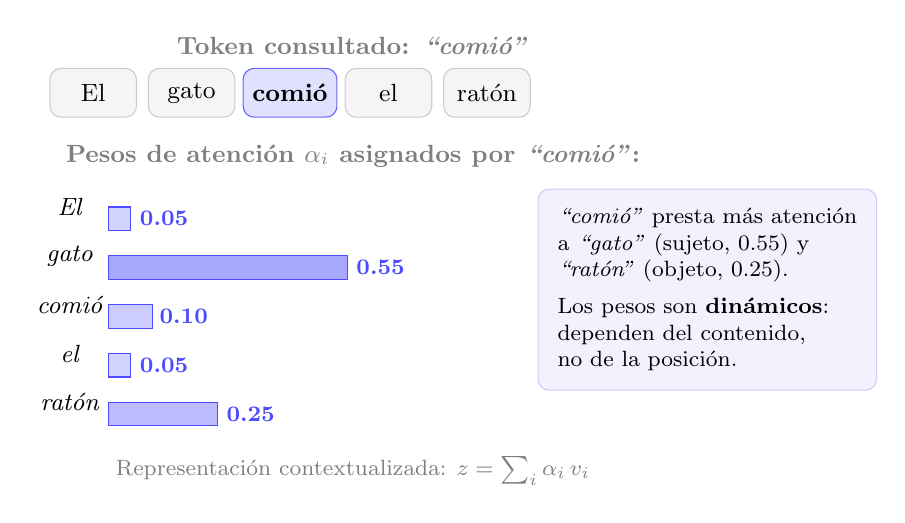
\begin{tikzpicture}[
    word/.style={draw=gray!40, rounded corners, fill=gray!8,
                 minimum width=1.1cm, minimum height=0.62cm, font=\small},
    focus/.style={draw=blue!60, rounded corners, fill=blue!12,
                  minimum width=1.1cm, minimum height=0.62cm,
                  font=\small\bfseries},
    weight/.style={font=\footnotesize\bfseries},
    bar/.style={fill=blue!50, draw=blue!70}
]

\node[font=\small\bfseries, gray] at (3.3, 5.6)
    {Token consultado: \textit{``comi\'o''}};

\node[word]  at (0*1.25, 5.0) {El};
\node[word]  at (1*1.25, 5.0) {gato};
\node[focus] at (2*1.25, 5.0) {comi\'o};
\node[word]  at (3*1.25, 5.0) {el};
\node[word]  at (4*1.25, 5.0) {rat\'on};

\node[font=\small\bfseries, gray] at (3.3, 4.2)
    {Pesos de atenci\'on $\alpha_i$ asignados por \textit{``comi\'o''}:};

\node[font=\small\itshape] at (-0.3, 3.55) {El};
\fill[bar, fill opacity=0.35] (0.2, 3.25) rectangle (0.475, 3.55);
\node[weight, blue!70] at (0.9, 3.40) {0.05};

\node[font=\small\itshape] at (-0.3, 2.93) {gato};
\fill[bar, fill opacity=0.685] (0.2, 2.63) rectangle (3.225, 2.93);
\node[weight, blue!70] at (3.65, 2.78) {0.55};

\node[font=\small\itshape] at (-0.3, 2.31) {comi\'o};
\fill[bar, fill opacity=0.40] (0.2, 2.01) rectangle (0.75, 2.31);
\node[weight, blue!70] at (1.15, 2.16) {0.10};

\node[font=\small\itshape] at (-0.3, 1.69) {el};
\fill[bar, fill opacity=0.35] (0.2, 1.39) rectangle (0.475, 1.69);
\node[weight, blue!70] at (0.9, 1.54) {0.05};

\node[font=\small\itshape] at (-0.3, 1.07) {rat\'on};
\fill[bar, fill opacity=0.525] (0.2, 0.77) rectangle (1.575, 1.07);
\node[weight, blue!70] at (2.0, 0.92) {0.25};

\node[draw=blue!20, fill=blue!5, rounded corners, font=\footnotesize,
      inner sep=7pt, align=left] at (7.8, 2.5)
    {\textit{``comi\'o''} presta m\'as atenci\'on\\
     a \textit{``gato''} (sujeto, 0.55) y\\
     \textit{``rat\'on''} (objeto, 0.25).\\[4pt]
     Los pesos son \textbf{din\'amicos}:\\
     dependen del contenido,\\
     no de la posici\'on.};

\node[font=\footnotesize, gray] at (3.3, 0.2)
    {Representaci\'on contextualizada:
     $\bm{z} = \sum_i \alpha_i \, \bm{v}_i$};

\end{tikzpicture}
\caption{Intuici\'on del mecanismo de atenci\'on. Para el token
\textit{comi\'o}, la atenci\'on calcula un peso $\alpha_i$ para cada
token de la secuencia. La representaci\'on final es una suma ponderada
de los valores, donde los pesos reflejan la relevancia sem\'antica.}
\label{fig:atencion_intuicion}
\end{figure}

% ============================================================
\begin{figure}[H]
\centering
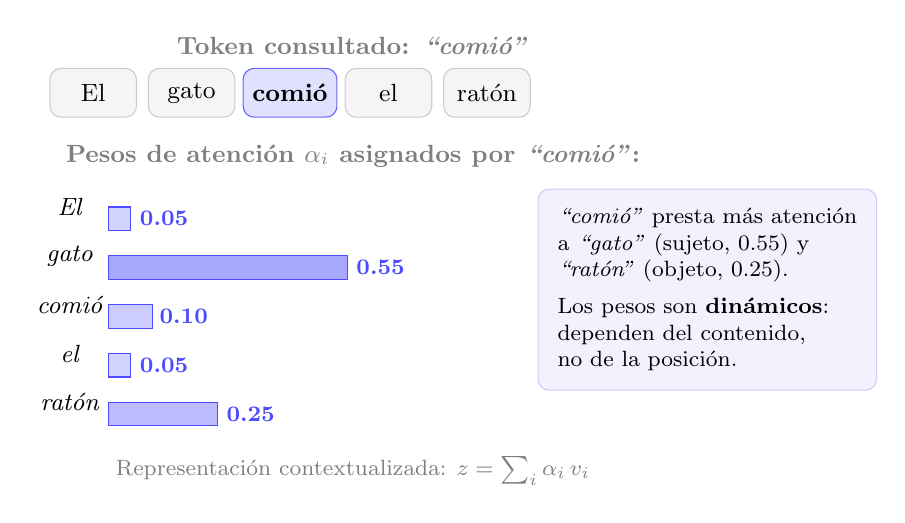
\begin{tikzpicture}[
    word/.style={draw=gray!40, rounded corners, fill=gray!8,
                 minimum width=1.1cm, minimum height=0.62cm, font=\small},
    focus/.style={draw=blue!60, rounded corners, fill=blue!12,
                  minimum width=1.1cm, minimum height=0.62cm,
                  font=\small\bfseries},
    weight/.style={font=\footnotesize\bfseries},
    bar/.style={fill=blue!50, draw=blue!70}
]

\node[font=\small\bfseries, gray] at (3.3, 5.6)
    {Token consultado: \textit{``comi\'o''}};

\node[word]  at (0*1.25, 5.0) {El};
\node[word]  at (1*1.25, 5.0) {gato};
\node[focus] at (2*1.25, 5.0) {comi\'o};
\node[word]  at (3*1.25, 5.0) {el};
\node[word]  at (4*1.25, 5.0) {rat\'on};

\node[font=\small\bfseries, gray] at (3.3, 4.2)
    {Pesos de atenci\'on $\alpha_i$ asignados por \textit{``comi\'o''}:};

\node[font=\small\itshape] at (-0.3, 3.55) {El};
\fill[bar, fill opacity=0.35] (0.2, 3.25) rectangle (0.475, 3.55);
\node[weight, blue!70] at (0.9, 3.40) {0.05};

\node[font=\small\itshape] at (-0.3, 2.93) {gato};
\fill[bar, fill opacity=0.685] (0.2, 2.63) rectangle (3.225, 2.93);
\node[weight, blue!70] at (3.65, 2.78) {0.55};

\node[font=\small\itshape] at (-0.3, 2.31) {comi\'o};
\fill[bar, fill opacity=0.40] (0.2, 2.01) rectangle (0.75, 2.31);
\node[weight, blue!70] at (1.15, 2.16) {0.10};

\node[font=\small\itshape] at (-0.3, 1.69) {el};
\fill[bar, fill opacity=0.35] (0.2, 1.39) rectangle (0.475, 1.69);
\node[weight, blue!70] at (0.9, 1.54) {0.05};

\node[font=\small\itshape] at (-0.3, 1.07) {rat\'on};
\fill[bar, fill opacity=0.525] (0.2, 0.77) rectangle (1.575, 1.07);
\node[weight, blue!70] at (2.0, 0.92) {0.25};

\node[draw=blue!20, fill=blue!5, rounded corners, font=\footnotesize,
      inner sep=7pt, align=left] at (7.8, 2.5)
    {\textit{``comi\'o''} presta m\'as atenci\'on\\
     a \textit{``gato''} (sujeto, 0.55) y\\
     \textit{``rat\'on''} (objeto, 0.25).\\[4pt]
     Los pesos son \textbf{din\'amicos}:\\
     dependen del contenido,\\
     no de la posici\'on.};

\node[font=\footnotesize, gray] at (3.3, 0.2)
    {Representaci\'on contextualizada:
     $\bm{z} = \sum_i \alpha_i \, \bm{v}_i$};

\end{tikzpicture}
\caption{Intuici\'on del mecanismo de atenci\'on. Para el token
\textit{comi\'o}, la atenci\'on calcula un peso $\alpha_i$ para cada
token de la secuencia. La representaci\'on final es una suma ponderada
de los valores, donde los pesos reflejan la relevancia sem\'antica.}
\label{fig:atencion_intuicion}
\end{figure}


Tres propiedades de este mecanismo lo distinguen radicalmente de los modelos
clásicos:

\begin{enumerate}
    \item \textbf{Global:} todos los tokens pueden relacionarse con todos,
    sin restricción de distancia.
    \item \textbf{Dinámico:} los pesos $\alpha_{ij}$ se calculan en función
    del contenido de la secuencia, no son parámetros fijos.
    \item \textbf{Paralelo:} el cómputo de todos los $\alpha_{ij}$ puede
    realizarse simultáneamente, sin procesamiento secuencial.
\end{enumerate}

%------------------------------------------------------------
\subsection{De la intuición a las matrices: Q, K y V}
\label{subsec:qkv}

La implementación práctica del mecanismo requiere operacionalizar la noción
de relevancia entre tokens. Vaswani et al.~\cite{vaswani2017attention}
proponen una analogía con los sistemas de recuperación de información: un
token emite una \textit{consulta} sobre qué necesita, el resto de los tokens
expone sus \textit{claves} (qué ofrecen), y la similitud entre consulta y
claves determina qué \textit{valores} se recuperan.

Concretamente, a partir de la representación de entrada $\bm{x}_i$ de cada
token se generan tres vectores mediante proyecciones lineales aprendidas:

\begin{align}
    \bm{q}_i &= W_Q\, \bm{x}_i \quad \in \mathbb{R}^{d_k}
    \quad \text{(\textit{query}: qué busca este token)} \\
    \bm{k}_j &= W_K\, \bm{x}_j \quad \in \mathbb{R}^{d_k}
    \quad \text{(\textit{key}: qué ofrece cada token)}   \\
    \bm{v}_j &= W_V\, \bm{x}_j \quad \in \mathbb{R}^{d_v}
    \quad \text{(\textit{value}: qué información aporta)}
\end{align}

\noindent donde $W_Q, W_K \in \mathbb{R}^{d_k \times d_{\text{model}}}$ y
$W_V \in \mathbb{R}^{d_v \times d_{\text{model}}}$ son matrices de peso
aprendidas. La relevancia entre los tokens $i$ y $j$ se mide mediante el
producto escalar $\bm{q}_i \cdot \bm{k}_j^\top$.

% ============================================================
% fig_qkv.tex: Mecanismo Q, K, V
% Uso: % ============================================================
% fig_qkv.tex: Mecanismo Q, K, V
% Uso: % ============================================================
% fig_qkv.tex: Mecanismo Q, K, V
% Uso: \input{figures/fig_qkv}
% ============================================================
\begin{figure}[H]
\centering
\begin{tikzpicture}[
    vec/.style={draw, rounded corners, minimum width=1.0cm,
                minimum height=0.55cm, font=\footnotesize, inner sep=3pt},
    q/.style={vec, fill=blue!15,  draw=blue!50},
    k/.style={vec, fill=red!12,   draw=red!45},
    v/.style={vec, fill=green!12, draw=green!50!black},
    op/.style={draw=gray!50, fill=gray!8, rounded corners,
               minimum width=1.1cm, minimum height=0.55cm,
               font=\footnotesize, align=center}
]

% ── Entrada ──────────────────────────────────────────────────
\node[vec, fill=gray!12, draw=gray!50, minimum width=2.0cm]
    (x) at (0, 0) {$\bm{x}_i \in \mathbb{R}^{d_{\text{model}}}$};

% ── Proyecciones ─────────────────────────────────────────────
\node[q, minimum width=1.5cm] (q) at (-2.8, -1.8)
    {$\bm{q}_i = W_Q \bm{x}_i$};
\node[k, minimum width=1.5cm] (k) at ( 0.0, -1.8)
    {$\bm{k}_j = W_K \bm{x}_j$};
\node[v, minimum width=1.5cm] (v) at ( 2.8, -1.8)
    {$\bm{v}_j = W_V \bm{x}_j$};

\draw[-{Stealth}, thick, blue!60]  (x.south) -- ++(-2.8,0) -- (q.north);
\draw[-{Stealth}, thick, red!50]   (x.south) -- (k.north);
\draw[-{Stealth}, thick, green!60!black] (x.south) -- ++(2.8,0) -- (v.north);

\node[blue!60,  font=\tiny] at (-1.8,-0.8) {$W_Q$};
\node[red!50,   font=\tiny] at ( 0.3,-0.9) {$W_K$};
\node[green!60!black, font=\tiny] at (1.8,-0.8) {$W_V$};

% ── Producto Q·K^T ───────────────────────────────────────────
\node[op] (dot) at (-1.4, -3.3) {$\bm{q}_i \cdot \bm{k}_j^{\top}$};
\draw[-{Stealth}, thick, gray] (q.south) -- ++(0,-0.7) -| (dot.north);
\draw[-{Stealth}, thick, gray] (k.south) -- ++(0,-0.7) -| (dot.north);

% ── Escalado ─────────────────────────────────────────────────
\node[op] (scale) at (-1.4, -4.5) {$/\sqrt{d_k}$};
\draw[-{Stealth}, thick] (dot) -- (scale);

% ── Softmax ──────────────────────────────────────────────────
\node[op, fill=orange!10, draw=orange!50] (softmax) at (-1.4, -5.7) {softmax};
\draw[-{Stealth}, thick] (scale) -- (softmax);
\node[font=\footnotesize\bfseries, orange!70] at (0.2,-5.7) {$\alpha_{ij}$};

% ── Suma ponderada ───────────────────────────────────────────
\node[op, fill=green!8, draw=green!50!black] (out) at (1.4, -7.0)
    {$\sum_j \alpha_{ij}\,\bm{v}_j$};
\draw[-{Stealth}, thick, orange!60]    (softmax.south) -- ++(0,-0.6) -| (out.north);
\draw[-{Stealth}, thick, green!60!black] (v.south)     -- ++(0,-4.5) -- (out.north);

% ── Salida ───────────────────────────────────────────────────
\node[vec, fill=purple!10, draw=purple!40, minimum width=1.8cm]
    (z) at (1.4, -8.2) {$\bm{z}_i \in \mathbb{R}^{d_v}$};
\draw[-{Stealth}, thick] (out) -- (z);
\node[font=\footnotesize, gray, align=center] at (3.4,-8.2)
    {representaci\'on\\contextualizada};

% ── Fórmula ──────────────────────────────────────────────────
\node[draw=blue!20, fill=blue!5, rounded corners, font=\small,
      inner sep=7pt, align=center] at (5.5, -4.5)
    {$\text{Attention}(Q,K,V)$\\[4pt]
     $=\,\text{softmax}\!\left(\dfrac{QK^{\top}}{\sqrt{d_k}}\right)V$};

\end{tikzpicture}
\caption{Mecanismo de atenci\'on de producto escalar escalado. A partir de
$\bm{x}_i$ se generan tres proyecciones: consulta $\bm{q}_i$, clave
$\bm{k}_j$ y valor $\bm{v}_j$. El producto $\bm{q}_i \cdot \bm{k}_j^\top$
mide la afinidad, se escala por $\sqrt{d_k}$ y se normaliza con softmax
para obtener los pesos $\alpha_{ij}$. La salida $\bm{z}_i$ es la suma
ponderada de los valores~\cite{vaswani2017attention}.}
\label{fig:qkv}
\end{figure}

% ============================================================
\begin{figure}[H]
\centering
\begin{tikzpicture}[
    vec/.style={draw, rounded corners, minimum width=1.0cm,
                minimum height=0.55cm, font=\footnotesize, inner sep=3pt},
    q/.style={vec, fill=blue!15,  draw=blue!50},
    k/.style={vec, fill=red!12,   draw=red!45},
    v/.style={vec, fill=green!12, draw=green!50!black},
    op/.style={draw=gray!50, fill=gray!8, rounded corners,
               minimum width=1.1cm, minimum height=0.55cm,
               font=\footnotesize, align=center}
]

% ── Entrada ──────────────────────────────────────────────────
\node[vec, fill=gray!12, draw=gray!50, minimum width=2.0cm]
    (x) at (0, 0) {$\bm{x}_i \in \mathbb{R}^{d_{\text{model}}}$};

% ── Proyecciones ─────────────────────────────────────────────
\node[q, minimum width=1.5cm] (q) at (-2.8, -1.8)
    {$\bm{q}_i = W_Q \bm{x}_i$};
\node[k, minimum width=1.5cm] (k) at ( 0.0, -1.8)
    {$\bm{k}_j = W_K \bm{x}_j$};
\node[v, minimum width=1.5cm] (v) at ( 2.8, -1.8)
    {$\bm{v}_j = W_V \bm{x}_j$};

\draw[-{Stealth}, thick, blue!60]  (x.south) -- ++(-2.8,0) -- (q.north);
\draw[-{Stealth}, thick, red!50]   (x.south) -- (k.north);
\draw[-{Stealth}, thick, green!60!black] (x.south) -- ++(2.8,0) -- (v.north);

\node[blue!60,  font=\tiny] at (-1.8,-0.8) {$W_Q$};
\node[red!50,   font=\tiny] at ( 0.3,-0.9) {$W_K$};
\node[green!60!black, font=\tiny] at (1.8,-0.8) {$W_V$};

% ── Producto Q·K^T ───────────────────────────────────────────
\node[op] (dot) at (-1.4, -3.3) {$\bm{q}_i \cdot \bm{k}_j^{\top}$};
\draw[-{Stealth}, thick, gray] (q.south) -- ++(0,-0.7) -| (dot.north);
\draw[-{Stealth}, thick, gray] (k.south) -- ++(0,-0.7) -| (dot.north);

% ── Escalado ─────────────────────────────────────────────────
\node[op] (scale) at (-1.4, -4.5) {$/\sqrt{d_k}$};
\draw[-{Stealth}, thick] (dot) -- (scale);

% ── Softmax ──────────────────────────────────────────────────
\node[op, fill=orange!10, draw=orange!50] (softmax) at (-1.4, -5.7) {softmax};
\draw[-{Stealth}, thick] (scale) -- (softmax);
\node[font=\footnotesize\bfseries, orange!70] at (0.2,-5.7) {$\alpha_{ij}$};

% ── Suma ponderada ───────────────────────────────────────────
\node[op, fill=green!8, draw=green!50!black] (out) at (1.4, -7.0)
    {$\sum_j \alpha_{ij}\,\bm{v}_j$};
\draw[-{Stealth}, thick, orange!60]    (softmax.south) -- ++(0,-0.6) -| (out.north);
\draw[-{Stealth}, thick, green!60!black] (v.south)     -- ++(0,-4.5) -- (out.north);

% ── Salida ───────────────────────────────────────────────────
\node[vec, fill=purple!10, draw=purple!40, minimum width=1.8cm]
    (z) at (1.4, -8.2) {$\bm{z}_i \in \mathbb{R}^{d_v}$};
\draw[-{Stealth}, thick] (out) -- (z);
\node[font=\footnotesize, gray, align=center] at (3.4,-8.2)
    {representaci\'on\\contextualizada};

% ── Fórmula ──────────────────────────────────────────────────
\node[draw=blue!20, fill=blue!5, rounded corners, font=\small,
      inner sep=7pt, align=center] at (5.5, -4.5)
    {$\text{Attention}(Q,K,V)$\\[4pt]
     $=\,\text{softmax}\!\left(\dfrac{QK^{\top}}{\sqrt{d_k}}\right)V$};

\end{tikzpicture}
\caption{Mecanismo de atenci\'on de producto escalar escalado. A partir de
$\bm{x}_i$ se generan tres proyecciones: consulta $\bm{q}_i$, clave
$\bm{k}_j$ y valor $\bm{v}_j$. El producto $\bm{q}_i \cdot \bm{k}_j^\top$
mide la afinidad, se escala por $\sqrt{d_k}$ y se normaliza con softmax
para obtener los pesos $\alpha_{ij}$. La salida $\bm{z}_i$ es la suma
ponderada de los valores~\cite{vaswani2017attention}.}
\label{fig:qkv}
\end{figure}

% ============================================================
\begin{figure}[H]
\centering
\begin{tikzpicture}[
    vec/.style={draw, rounded corners, minimum width=1.0cm,
                minimum height=0.55cm, font=\footnotesize, inner sep=3pt},
    q/.style={vec, fill=blue!15,  draw=blue!50},
    k/.style={vec, fill=red!12,   draw=red!45},
    v/.style={vec, fill=green!12, draw=green!50!black},
    op/.style={draw=gray!50, fill=gray!8, rounded corners,
               minimum width=1.1cm, minimum height=0.55cm,
               font=\footnotesize, align=center}
]

% ── Entrada ──────────────────────────────────────────────────
\node[vec, fill=gray!12, draw=gray!50, minimum width=2.0cm]
    (x) at (0, 0) {$\bm{x}_i \in \mathbb{R}^{d_{\text{model}}}$};

% ── Proyecciones ─────────────────────────────────────────────
\node[q, minimum width=1.5cm] (q) at (-2.8, -1.8)
    {$\bm{q}_i = W_Q \bm{x}_i$};
\node[k, minimum width=1.5cm] (k) at ( 0.0, -1.8)
    {$\bm{k}_j = W_K \bm{x}_j$};
\node[v, minimum width=1.5cm] (v) at ( 2.8, -1.8)
    {$\bm{v}_j = W_V \bm{x}_j$};

\draw[-{Stealth}, thick, blue!60]  (x.south) -- ++(-2.8,0) -- (q.north);
\draw[-{Stealth}, thick, red!50]   (x.south) -- (k.north);
\draw[-{Stealth}, thick, green!60!black] (x.south) -- ++(2.8,0) -- (v.north);

\node[blue!60,  font=\tiny] at (-1.8,-0.8) {$W_Q$};
\node[red!50,   font=\tiny] at ( 0.3,-0.9) {$W_K$};
\node[green!60!black, font=\tiny] at (1.8,-0.8) {$W_V$};

% ── Producto Q·K^T ───────────────────────────────────────────
\node[op] (dot) at (-1.4, -3.3) {$\bm{q}_i \cdot \bm{k}_j^{\top}$};
\draw[-{Stealth}, thick, gray] (q.south) -- ++(0,-0.7) -| (dot.north);
\draw[-{Stealth}, thick, gray] (k.south) -- ++(0,-0.7) -| (dot.north);

% ── Escalado ─────────────────────────────────────────────────
\node[op] (scale) at (-1.4, -4.5) {$/\sqrt{d_k}$};
\draw[-{Stealth}, thick] (dot) -- (scale);

% ── Softmax ──────────────────────────────────────────────────
\node[op, fill=orange!10, draw=orange!50] (softmax) at (-1.4, -5.7) {softmax};
\draw[-{Stealth}, thick] (scale) -- (softmax);
\node[font=\footnotesize\bfseries, orange!70] at (0.2,-5.7) {$\alpha_{ij}$};

% ── Suma ponderada ───────────────────────────────────────────
\node[op, fill=green!8, draw=green!50!black] (out) at (1.4, -7.0)
    {$\sum_j \alpha_{ij}\,\bm{v}_j$};
\draw[-{Stealth}, thick, orange!60]    (softmax.south) -- ++(0,-0.6) -| (out.north);
\draw[-{Stealth}, thick, green!60!black] (v.south)     -- ++(0,-4.5) -- (out.north);

% ── Salida ───────────────────────────────────────────────────
\node[vec, fill=purple!10, draw=purple!40, minimum width=1.8cm]
    (z) at (1.4, -8.2) {$\bm{z}_i \in \mathbb{R}^{d_v}$};
\draw[-{Stealth}, thick] (out) -- (z);
\node[font=\footnotesize, gray, align=center] at (3.4,-8.2)
    {representaci\'on\\contextualizada};

% ── Fórmula ──────────────────────────────────────────────────
\node[draw=blue!20, fill=blue!5, rounded corners, font=\small,
      inner sep=7pt, align=center] at (5.5, -4.5)
    {$\text{Attention}(Q,K,V)$\\[4pt]
     $=\,\text{softmax}\!\left(\dfrac{QK^{\top}}{\sqrt{d_k}}\right)V$};

\end{tikzpicture}
\caption{Mecanismo de atenci\'on de producto escalar escalado. A partir de
$\bm{x}_i$ se generan tres proyecciones: consulta $\bm{q}_i$, clave
$\bm{k}_j$ y valor $\bm{v}_j$. El producto $\bm{q}_i \cdot \bm{k}_j^\top$
mide la afinidad, se escala por $\sqrt{d_k}$ y se normaliza con softmax
para obtener los pesos $\alpha_{ij}$. La salida $\bm{z}_i$ es la suma
ponderada de los valores~\cite{vaswani2017attention}.}
\label{fig:qkv}
\end{figure}


%------------------------------------------------------------
\subsection{Atención de producto escalar escalado}
\label{subsec:scaled_dot_product}

Operando sobre toda la secuencia de forma matricial, las consultas, claves
y valores se apilan en matrices $Q \in \mathbb{R}^{n \times d_k}$,
$K \in \mathbb{R}^{n \times d_k}$ y $V \in \mathbb{R}^{n \times d_v}$.
La atención se computa entonces como:

\begin{equation}
    \text{Attention}(Q, K, V) =
    \text{softmax}\!\left(\frac{QK^{\top}}{\sqrt{d_k}}\right) V
    \label{eq:attention}
\end{equation}

Cada componente cumple un rol preciso:

\begin{itemize}
    \item $QK^{\top}$: matriz de \textit{scores} de afinidad entre todos los
    pares de tokens. El elemento $(i,j)$ mide cuánto se parece la consulta
    del token $i$ a la clave del token $j$.

    \item $1/\sqrt{d_k}$: factor de escala que estabiliza el entrenamiento.
    Para dimensiones $d_k$ grandes, los productos escalares crecen en
    magnitud y empujan a la función softmax hacia regiones de gradiente
    muy pequeño; dividir por $\sqrt{d_k}$ corrige este efecto~\cite{vaswani2017attention}.

    \item $\text{softmax}(\cdot)$: normaliza los scores por fila, produciendo
    pesos $\alpha_{ij} \in (0,1)$ con $\sum_j \alpha_{ij} = 1$, interpretables
    como una distribución de probabilidad sobre la secuencia.

    \item $V$: los pesos se aplican sobre los valores, produciendo para cada
    token una representación contextualizada que integra información de toda
    la secuencia ponderada por relevancia.
\end{itemize}

%------------------------------------------------------------
\subsection{Ejemplo numérico paso a paso}
\label{subsec:atencion_ejemplo}

Para concretar el mecanismo, se presenta un ejemplo con la secuencia
\textit{gato–comió–ratón} ($n = 3$ tokens, $d_k = d_v = 2$). Los valores
numéricos son ilustrativos y están elegidos para producir un resultado
interpretable.

% ============================================================
% fig_atencion_ejemplo.tex: Ejemplo numérico Q, K, V (3 tokens)
% Uso: % ============================================================
% fig_atencion_ejemplo.tex: Ejemplo numérico Q, K, V (3 tokens)
% Uso: % ============================================================
% fig_atencion_ejemplo.tex: Ejemplo numérico Q, K, V (3 tokens)
% Uso: \input{figures/fig_atencion_ejemplo}
% ============================================================
\begin{figure}[H]
\centering
\begin{tikzpicture}[
    cell/.style={draw=gray!40, minimum width=1.1cm, minimum height=0.60cm,
                 font=\footnotesize, inner sep=2pt},
    hdr/.style={font=\footnotesize\bfseries},
    qc/.style={fill=blue!12},
    kc/.style={fill=red!10},
    vc/.style={fill=green!10},
    sc/.style={fill=orange!12},
    ac/.style={fill=purple!10},
    zc/.style={fill=teal!10},
    stepnode/.style={font=\small\bfseries, blue!70}
]

\node[font=\small\bfseries, gray] at (5.0, 8.5)
    {Secuencia: \textit{gato} $(t_1)$ \quad \textit{comi\'o} $(t_2)$ \quad
     \textit{rat\'on} $(t_3)$ \quad $|$ \quad $d_k = d_v = 2$};

% ── PASO 1: Matrices Q, K, V ─────────────────────────────────
\node[stepnode] at (-0.5, 7.7) {Paso 1};
\foreach \lbl/\x in {Q/1.5, K/4.0, V/6.5}{
    \node[hdr] at (\x, 7.7) {$\lbl$};
}
\foreach \lbl/\y in {$t_1$/7.1, $t_2$/6.45, $t_3$/5.80}{
    \node[font=\footnotesize] at (0.3, \y) {\lbl};
}
% Q
\node[cell,qc] at (1.1,7.10){1.0}; \node[cell,qc] at (2.0,7.10){0.0};
\node[cell,qc] at (1.1,6.45){0.0}; \node[cell,qc] at (2.0,6.45){1.0};
\node[cell,qc] at (1.1,5.80){1.0}; \node[cell,qc] at (2.0,5.80){1.0};
% K
\node[cell,kc] at (3.6,7.10){1.0}; \node[cell,kc] at (4.5,7.10){0.0};
\node[cell,kc] at (3.6,6.45){1.0}; \node[cell,kc] at (4.5,6.45){1.0};
\node[cell,kc] at (3.6,5.80){0.0}; \node[cell,kc] at (4.5,5.80){1.0};
% V
\node[cell,vc] at (6.1,7.10){1.0}; \node[cell,vc] at (7.0,7.10){0.0};
\node[cell,vc] at (6.1,6.45){0.5}; \node[cell,vc] at (7.0,6.45){0.5};
\node[cell,vc] at (6.1,5.80){0.0}; \node[cell,vc] at (7.0,5.80){1.0};

% ── PASO 2: Scores ───────────────────────────────────────────
\node[stepnode] at (-0.5, 4.85) {Paso 2};
\node[hdr, align=center] at (1.8, 4.85) {$S = QK^{\top}/\sqrt{2}$};
\foreach \lbl/\x in {$t_1$/1.1, $t_2$/2.2, $t_3$/3.3}{
    \node[font=\footnotesize] at (\x, 4.35) {\lbl};
}
\foreach \lbl/\y in {$t_1$/3.85, $t_2$/3.20, $t_3$/2.55}{
    \node[font=\footnotesize] at (0.3, \y) {\lbl};
}
\node[cell,sc] at (1.1,3.85){0.71}; \node[cell,sc] at (2.2,3.85){0.71}; \node[cell,sc] at (3.3,3.85){0.00};
\node[cell,sc] at (1.1,3.20){0.00}; \node[cell,sc] at (2.2,3.20){0.71}; \node[cell,sc] at (3.3,3.20){0.71};
\node[cell,sc] at (1.1,2.55){0.71}; \node[cell,sc] at (2.2,2.55){1.41}; \node[cell,sc] at (3.3,2.55){0.71};

% ── Flecha softmax ───────────────────────────────────────────
\draw[-{Stealth}, thick, gray!60] (3.8, 3.2) -- (4.6, 3.2);
\node[font=\tiny, gray, align=center] at (4.2, 3.5) {softmax\\por fila};

% ── PASO 3: Pesos α ──────────────────────────────────────────
\node[stepnode] at (5.2, 4.85) {Paso 3};
\node[hdr, align=center] at (6.8, 4.85) {$A = \text{softmax}(S)$};
\foreach \lbl/\x in {$t_1$/5.6, $t_2$/6.7, $t_3$/7.8}{
    \node[font=\footnotesize] at (\x, 4.35) {\lbl};
}
\foreach \lbl/\y in {$t_1$/3.85, $t_2$/3.20, $t_3$/2.55}{
    \node[font=\footnotesize] at (4.9, \y) {\lbl};
}
\node[cell,ac] at (5.6,3.85){0.40}; \node[cell,ac] at (6.7,3.85){0.40}; \node[cell,ac] at (7.8,3.85){0.20};
\node[cell,ac] at (5.6,3.20){0.20}; \node[cell,ac] at (6.7,3.20){0.40}; \node[cell,ac] at (7.8,3.20){0.40};
\node[cell,ac] at (5.6,2.55){0.25}; \node[cell,ac] at (6.7,2.55){0.50}; \node[cell,ac] at (7.8,2.55){0.25};

% ── PASO 4: Z = A·V ──────────────────────────────────────────
\node[stepnode] at (3.0, 1.85) {Paso 4};
\node[hdr, align=center] at (5.2, 1.85) {$Z = A \cdot V$};
\foreach \lbl/\x in {dim1/4.6, dim2/5.7}{
    \node[font=\footnotesize] at (\x, 1.35) {\lbl};
}
\foreach \lbl/\y in {$z_1$/0.90, $z_2$/0.25, $z_3$/-0.40}{
    \node[font=\footnotesize] at (3.8, \y) {\lbl};
}
\node[cell,zc] at (4.6, 0.90){0.60}; \node[cell,zc] at (5.7, 0.90){0.40};
\node[cell,zc] at (4.6, 0.25){0.40}; \node[cell,zc] at (5.7, 0.25){0.60};
\node[cell,zc] at (4.6,-0.40){0.50}; \node[cell,zc] at (5.7,-0.40){0.50};

\draw[-{Stealth}, thick, gray!60]
    (7.3, 2.55) -- ++(0,-0.4) -- ++(-1.1,0) -- ++(0,-0.4);
\node[font=\tiny, gray] at (8.3, 2.1) {$Z = A \cdot V$};

\node[draw=gray!30, fill=gray!5, rounded corners, font=\tiny,
      inner sep=5pt, align=left] at (8.8, 0.3)
    {Fila $i$ de $Z$: representaci\'on de $t_i$\\
     contextualizada por toda la secuencia.};

\end{tikzpicture}
\caption{Ejemplo num\'erico de atenci\'on escalada con 3 tokens ($d_k=d_v=2$).
\textbf{Paso 1:} matrices $Q$, $K$, $V$.
\textbf{Paso 2:} scores $S=QK^\top/\sqrt{d_k}$.
\textbf{Paso 3:} pesos $\alpha_{ij}$ tras softmax por fila.
\textbf{Paso 4:} salida $Z=AV$. Valores ilustrativos.}
\label{fig:atencion_ejemplo}
\end{figure}

% ============================================================
\begin{figure}[H]
\centering
\begin{tikzpicture}[
    cell/.style={draw=gray!40, minimum width=1.1cm, minimum height=0.60cm,
                 font=\footnotesize, inner sep=2pt},
    hdr/.style={font=\footnotesize\bfseries},
    qc/.style={fill=blue!12},
    kc/.style={fill=red!10},
    vc/.style={fill=green!10},
    sc/.style={fill=orange!12},
    ac/.style={fill=purple!10},
    zc/.style={fill=teal!10},
    stepnode/.style={font=\small\bfseries, blue!70}
]

\node[font=\small\bfseries, gray] at (5.0, 8.5)
    {Secuencia: \textit{gato} $(t_1)$ \quad \textit{comi\'o} $(t_2)$ \quad
     \textit{rat\'on} $(t_3)$ \quad $|$ \quad $d_k = d_v = 2$};

% ── PASO 1: Matrices Q, K, V ─────────────────────────────────
\node[stepnode] at (-0.5, 7.7) {Paso 1};
\foreach \lbl/\x in {Q/1.5, K/4.0, V/6.5}{
    \node[hdr] at (\x, 7.7) {$\lbl$};
}
\foreach \lbl/\y in {$t_1$/7.1, $t_2$/6.45, $t_3$/5.80}{
    \node[font=\footnotesize] at (0.3, \y) {\lbl};
}
% Q
\node[cell,qc] at (1.1,7.10){1.0}; \node[cell,qc] at (2.0,7.10){0.0};
\node[cell,qc] at (1.1,6.45){0.0}; \node[cell,qc] at (2.0,6.45){1.0};
\node[cell,qc] at (1.1,5.80){1.0}; \node[cell,qc] at (2.0,5.80){1.0};
% K
\node[cell,kc] at (3.6,7.10){1.0}; \node[cell,kc] at (4.5,7.10){0.0};
\node[cell,kc] at (3.6,6.45){1.0}; \node[cell,kc] at (4.5,6.45){1.0};
\node[cell,kc] at (3.6,5.80){0.0}; \node[cell,kc] at (4.5,5.80){1.0};
% V
\node[cell,vc] at (6.1,7.10){1.0}; \node[cell,vc] at (7.0,7.10){0.0};
\node[cell,vc] at (6.1,6.45){0.5}; \node[cell,vc] at (7.0,6.45){0.5};
\node[cell,vc] at (6.1,5.80){0.0}; \node[cell,vc] at (7.0,5.80){1.0};

% ── PASO 2: Scores ───────────────────────────────────────────
\node[stepnode] at (-0.5, 4.85) {Paso 2};
\node[hdr, align=center] at (1.8, 4.85) {$S = QK^{\top}/\sqrt{2}$};
\foreach \lbl/\x in {$t_1$/1.1, $t_2$/2.2, $t_3$/3.3}{
    \node[font=\footnotesize] at (\x, 4.35) {\lbl};
}
\foreach \lbl/\y in {$t_1$/3.85, $t_2$/3.20, $t_3$/2.55}{
    \node[font=\footnotesize] at (0.3, \y) {\lbl};
}
\node[cell,sc] at (1.1,3.85){0.71}; \node[cell,sc] at (2.2,3.85){0.71}; \node[cell,sc] at (3.3,3.85){0.00};
\node[cell,sc] at (1.1,3.20){0.00}; \node[cell,sc] at (2.2,3.20){0.71}; \node[cell,sc] at (3.3,3.20){0.71};
\node[cell,sc] at (1.1,2.55){0.71}; \node[cell,sc] at (2.2,2.55){1.41}; \node[cell,sc] at (3.3,2.55){0.71};

% ── Flecha softmax ───────────────────────────────────────────
\draw[-{Stealth}, thick, gray!60] (3.8, 3.2) -- (4.6, 3.2);
\node[font=\tiny, gray, align=center] at (4.2, 3.5) {softmax\\por fila};

% ── PASO 3: Pesos α ──────────────────────────────────────────
\node[stepnode] at (5.2, 4.85) {Paso 3};
\node[hdr, align=center] at (6.8, 4.85) {$A = \text{softmax}(S)$};
\foreach \lbl/\x in {$t_1$/5.6, $t_2$/6.7, $t_3$/7.8}{
    \node[font=\footnotesize] at (\x, 4.35) {\lbl};
}
\foreach \lbl/\y in {$t_1$/3.85, $t_2$/3.20, $t_3$/2.55}{
    \node[font=\footnotesize] at (4.9, \y) {\lbl};
}
\node[cell,ac] at (5.6,3.85){0.40}; \node[cell,ac] at (6.7,3.85){0.40}; \node[cell,ac] at (7.8,3.85){0.20};
\node[cell,ac] at (5.6,3.20){0.20}; \node[cell,ac] at (6.7,3.20){0.40}; \node[cell,ac] at (7.8,3.20){0.40};
\node[cell,ac] at (5.6,2.55){0.25}; \node[cell,ac] at (6.7,2.55){0.50}; \node[cell,ac] at (7.8,2.55){0.25};

% ── PASO 4: Z = A·V ──────────────────────────────────────────
\node[stepnode] at (3.0, 1.85) {Paso 4};
\node[hdr, align=center] at (5.2, 1.85) {$Z = A \cdot V$};
\foreach \lbl/\x in {dim1/4.6, dim2/5.7}{
    \node[font=\footnotesize] at (\x, 1.35) {\lbl};
}
\foreach \lbl/\y in {$z_1$/0.90, $z_2$/0.25, $z_3$/-0.40}{
    \node[font=\footnotesize] at (3.8, \y) {\lbl};
}
\node[cell,zc] at (4.6, 0.90){0.60}; \node[cell,zc] at (5.7, 0.90){0.40};
\node[cell,zc] at (4.6, 0.25){0.40}; \node[cell,zc] at (5.7, 0.25){0.60};
\node[cell,zc] at (4.6,-0.40){0.50}; \node[cell,zc] at (5.7,-0.40){0.50};

\draw[-{Stealth}, thick, gray!60]
    (7.3, 2.55) -- ++(0,-0.4) -- ++(-1.1,0) -- ++(0,-0.4);
\node[font=\tiny, gray] at (8.3, 2.1) {$Z = A \cdot V$};

\node[draw=gray!30, fill=gray!5, rounded corners, font=\tiny,
      inner sep=5pt, align=left] at (8.8, 0.3)
    {Fila $i$ de $Z$: representaci\'on de $t_i$\\
     contextualizada por toda la secuencia.};

\end{tikzpicture}
\caption{Ejemplo num\'erico de atenci\'on escalada con 3 tokens ($d_k=d_v=2$).
\textbf{Paso 1:} matrices $Q$, $K$, $V$.
\textbf{Paso 2:} scores $S=QK^\top/\sqrt{d_k}$.
\textbf{Paso 3:} pesos $\alpha_{ij}$ tras softmax por fila.
\textbf{Paso 4:} salida $Z=AV$. Valores ilustrativos.}
\label{fig:atencion_ejemplo}
\end{figure}

% ============================================================
\begin{figure}[H]
\centering
\begin{tikzpicture}[
    cell/.style={draw=gray!40, minimum width=1.1cm, minimum height=0.60cm,
                 font=\footnotesize, inner sep=2pt},
    hdr/.style={font=\footnotesize\bfseries},
    qc/.style={fill=blue!12},
    kc/.style={fill=red!10},
    vc/.style={fill=green!10},
    sc/.style={fill=orange!12},
    ac/.style={fill=purple!10},
    zc/.style={fill=teal!10},
    stepnode/.style={font=\small\bfseries, blue!70}
]

\node[font=\small\bfseries, gray] at (5.0, 8.5)
    {Secuencia: \textit{gato} $(t_1)$ \quad \textit{comi\'o} $(t_2)$ \quad
     \textit{rat\'on} $(t_3)$ \quad $|$ \quad $d_k = d_v = 2$};

% ── PASO 1: Matrices Q, K, V ─────────────────────────────────
\node[stepnode] at (-0.5, 7.7) {Paso 1};
\foreach \lbl/\x in {Q/1.5, K/4.0, V/6.5}{
    \node[hdr] at (\x, 7.7) {$\lbl$};
}
\foreach \lbl/\y in {$t_1$/7.1, $t_2$/6.45, $t_3$/5.80}{
    \node[font=\footnotesize] at (0.3, \y) {\lbl};
}
% Q
\node[cell,qc] at (1.1,7.10){1.0}; \node[cell,qc] at (2.0,7.10){0.0};
\node[cell,qc] at (1.1,6.45){0.0}; \node[cell,qc] at (2.0,6.45){1.0};
\node[cell,qc] at (1.1,5.80){1.0}; \node[cell,qc] at (2.0,5.80){1.0};
% K
\node[cell,kc] at (3.6,7.10){1.0}; \node[cell,kc] at (4.5,7.10){0.0};
\node[cell,kc] at (3.6,6.45){1.0}; \node[cell,kc] at (4.5,6.45){1.0};
\node[cell,kc] at (3.6,5.80){0.0}; \node[cell,kc] at (4.5,5.80){1.0};
% V
\node[cell,vc] at (6.1,7.10){1.0}; \node[cell,vc] at (7.0,7.10){0.0};
\node[cell,vc] at (6.1,6.45){0.5}; \node[cell,vc] at (7.0,6.45){0.5};
\node[cell,vc] at (6.1,5.80){0.0}; \node[cell,vc] at (7.0,5.80){1.0};

% ── PASO 2: Scores ───────────────────────────────────────────
\node[stepnode] at (-0.5, 4.85) {Paso 2};
\node[hdr, align=center] at (1.8, 4.85) {$S = QK^{\top}/\sqrt{2}$};
\foreach \lbl/\x in {$t_1$/1.1, $t_2$/2.2, $t_3$/3.3}{
    \node[font=\footnotesize] at (\x, 4.35) {\lbl};
}
\foreach \lbl/\y in {$t_1$/3.85, $t_2$/3.20, $t_3$/2.55}{
    \node[font=\footnotesize] at (0.3, \y) {\lbl};
}
\node[cell,sc] at (1.1,3.85){0.71}; \node[cell,sc] at (2.2,3.85){0.71}; \node[cell,sc] at (3.3,3.85){0.00};
\node[cell,sc] at (1.1,3.20){0.00}; \node[cell,sc] at (2.2,3.20){0.71}; \node[cell,sc] at (3.3,3.20){0.71};
\node[cell,sc] at (1.1,2.55){0.71}; \node[cell,sc] at (2.2,2.55){1.41}; \node[cell,sc] at (3.3,2.55){0.71};

% ── Flecha softmax ───────────────────────────────────────────
\draw[-{Stealth}, thick, gray!60] (3.8, 3.2) -- (4.6, 3.2);
\node[font=\tiny, gray, align=center] at (4.2, 3.5) {softmax\\por fila};

% ── PASO 3: Pesos α ──────────────────────────────────────────
\node[stepnode] at (5.2, 4.85) {Paso 3};
\node[hdr, align=center] at (6.8, 4.85) {$A = \text{softmax}(S)$};
\foreach \lbl/\x in {$t_1$/5.6, $t_2$/6.7, $t_3$/7.8}{
    \node[font=\footnotesize] at (\x, 4.35) {\lbl};
}
\foreach \lbl/\y in {$t_1$/3.85, $t_2$/3.20, $t_3$/2.55}{
    \node[font=\footnotesize] at (4.9, \y) {\lbl};
}
\node[cell,ac] at (5.6,3.85){0.40}; \node[cell,ac] at (6.7,3.85){0.40}; \node[cell,ac] at (7.8,3.85){0.20};
\node[cell,ac] at (5.6,3.20){0.20}; \node[cell,ac] at (6.7,3.20){0.40}; \node[cell,ac] at (7.8,3.20){0.40};
\node[cell,ac] at (5.6,2.55){0.25}; \node[cell,ac] at (6.7,2.55){0.50}; \node[cell,ac] at (7.8,2.55){0.25};

% ── PASO 4: Z = A·V ──────────────────────────────────────────
\node[stepnode] at (3.0, 1.85) {Paso 4};
\node[hdr, align=center] at (5.2, 1.85) {$Z = A \cdot V$};
\foreach \lbl/\x in {dim1/4.6, dim2/5.7}{
    \node[font=\footnotesize] at (\x, 1.35) {\lbl};
}
\foreach \lbl/\y in {$z_1$/0.90, $z_2$/0.25, $z_3$/-0.40}{
    \node[font=\footnotesize] at (3.8, \y) {\lbl};
}
\node[cell,zc] at (4.6, 0.90){0.60}; \node[cell,zc] at (5.7, 0.90){0.40};
\node[cell,zc] at (4.6, 0.25){0.40}; \node[cell,zc] at (5.7, 0.25){0.60};
\node[cell,zc] at (4.6,-0.40){0.50}; \node[cell,zc] at (5.7,-0.40){0.50};

\draw[-{Stealth}, thick, gray!60]
    (7.3, 2.55) -- ++(0,-0.4) -- ++(-1.1,0) -- ++(0,-0.4);
\node[font=\tiny, gray] at (8.3, 2.1) {$Z = A \cdot V$};

\node[draw=gray!30, fill=gray!5, rounded corners, font=\tiny,
      inner sep=5pt, align=left] at (8.8, 0.3)
    {Fila $i$ de $Z$: representaci\'on de $t_i$\\
     contextualizada por toda la secuencia.};

\end{tikzpicture}
\caption{Ejemplo num\'erico de atenci\'on escalada con 3 tokens ($d_k=d_v=2$).
\textbf{Paso 1:} matrices $Q$, $K$, $V$.
\textbf{Paso 2:} scores $S=QK^\top/\sqrt{d_k}$.
\textbf{Paso 3:} pesos $\alpha_{ij}$ tras softmax por fila.
\textbf{Paso 4:} salida $Z=AV$. Valores ilustrativos.}
\label{fig:atencion_ejemplo}
\end{figure}


La fila $i$ de la salida $Z$ contiene la representación contextualizada
del token $i$. Por ejemplo, la fila de \textit{comió} ($t_2$) de la matriz de
pesos es $(0.20,\, 0.40,\, 0.40)$: el verbo reparte su atención por igual
entre sí mismo y \textit{ratón}, y le presta menos a \textit{gato}. Su
representación $z_2 = (0.40,\, 0.60)$ es entonces una mezcla de los valores
de los tres tokens en esas proporciones. Este resultado emerge del producto
escalar entre vectores, sin reglas explícitas. Los valores de $Q$, $K$ y $V$
son ilustrativos: en un modelo real los aprende el entrenamiento.

%------------------------------------------------------------
\subsection{Atención multi-cabeza}
\label{subsec:multihead}

Un único mecanismo de atención puede capturar un tipo de relación a la vez.
Sin embargo, una oración contiene simultáneamente relaciones sintácticas,
semánticas, de correferencia, posicionales, entre otras. La
\textit{atención multi-cabeza} (\textit{Multi-Head Attention}) resuelve
esto ejecutando $h$ mecanismos de atención en paralelo, cada uno con sus
propias matrices de proyección:

\begin{equation}
    \text{head}_l = \text{Attention}(Q W_Q^l,\; K W_K^l,\; V W_V^l)
    \qquad l = 1, \ldots, h
\end{equation}

Las salidas de cada cabeza se concatenan y se proyectan con una matriz
$W^O \in \mathbb{R}^{h d_v \times d_{\text{model}}}$:

\begin{equation}
    \text{MultiHead}(Q, K, V) =
    \text{Concat}(\text{head}_1, \ldots, \text{head}_h)\, W^O
\end{equation}

Para mantener el costo computacional constante, cada cabeza opera en un
subespacio de dimensión reducida: $d_k = d_v = d_{\text{model}} / h$.

% ============================================================
% fig_multihead.tex: Multi-Head Attention
% Uso: % ============================================================
% fig_multihead.tex: Multi-Head Attention
% Uso: % ============================================================
% fig_multihead.tex: Multi-Head Attention
% Uso: \input{figures/fig_multihead}
% ============================================================
\begin{figure}[H]
\centering
\begin{tikzpicture}[
    head/.style={draw, rounded corners, minimum width=1.5cm,
                 minimum height=0.7cm, font=\footnotesize\bfseries,
                 align=center},
    h1/.style={head, fill=blue!12,   draw=blue!50},
    h2/.style={head, fill=red!10,    draw=red!45},
    h3/.style={head, fill=green!10,  draw=green!50!black},
    h4/.style={head, fill=orange!10, draw=orange!50},
    box/.style={draw=gray!50, fill=gray!6, rounded corners,
                minimum width=5.5cm, minimum height=0.7cm,
                font=\small, align=center}
]

% ── Entrada ──────────────────────────────────────────────────
\node[box] (inp) at (3.5, 6.5)
    {Entrada $X \in \mathbb{R}^{n \times d_{\text{model}}}$};

% ── 4 cabezas ────────────────────────────────────────────────
\node[h1] (h1) at (0.7,  5.0) {Head 1\\$W_Q^1,W_K^1,W_V^1$};
\node[h2] (h2) at (2.5,  5.0) {Head 2\\$W_Q^2,W_K^2,W_V^2$};
\node[h3] (h3) at (4.3,  5.0) {Head 3\\$W_Q^3,W_K^3,W_V^3$};
\node[h4] (h4) at (6.1,  5.0) {Head 4\\$W_Q^4,W_K^4,W_V^4$};

\draw[-{Stealth}, thick, blue!50]        (inp.south) -| (h1.north);
\draw[-{Stealth}, thick, red!45]         (inp.south) -| (h2.north);
\draw[-{Stealth}, thick, green!50!black] (inp.south) -| (h3.north);
\draw[-{Stealth}, thick, orange!50]      (inp.south) -| (h4.north);

\node[font=\footnotesize, gray] at (3.5, 5.85)
    {proyecciones independientes ($d_k = d_{\text{model}}/h$)};

% ── Salidas ──────────────────────────────────────────────────
\node[h1, minimum height=0.55cm] (z1) at (0.7,  3.7) {$Z_1$};
\node[h2, minimum height=0.55cm] (z2) at (2.5,  3.7) {$Z_2$};
\node[h3, minimum height=0.55cm] (z3) at (4.3,  3.7) {$Z_3$};
\node[h4, minimum height=0.55cm] (z4) at (6.1,  3.7) {$Z_4$};

\draw[-{Stealth}, thick] (h1)--(z1);
\draw[-{Stealth}, thick] (h2)--(z2);
\draw[-{Stealth}, thick] (h3)--(z3);
\draw[-{Stealth}, thick] (h4)--(z4);

% ── Concatenación ────────────────────────────────────────────
\node[box, fill=yellow!8, draw=yellow!60!black] (concat) at (3.5, 2.6)
    {Concat$(Z_1, Z_2, Z_3, Z_4)$};
\draw[-{Stealth}, thick] (z1.south) |- (concat.west);
\draw[-{Stealth}, thick] (z2.south) -- (concat.north);
\draw[-{Stealth}, thick] (z3.south) -- (concat.north);
\draw[-{Stealth}, thick] (z4.south) |- (concat.east);

% ── Proyección final ─────────────────────────────────────────
\node[box, fill=purple!8, draw=purple!40] (proj) at (3.5, 1.5)
    {Proyecci\'on lineal $W^O$};
\draw[-{Stealth}, thick] (concat)--(proj);

% ── Salida ───────────────────────────────────────────────────
\node[box] (out) at (3.5, 0.5)
    {Salida $\in \mathbb{R}^{n \times d_{\text{model}}}$};
\draw[-{Stealth}, thick] (proj)--(out);

% ── Anotación ────────────────────────────────────────────────
\node[draw=blue!15, fill=blue!4, rounded corners, font=\footnotesize,
      inner sep=6pt, align=left] at (9.6, 3.8)
    {Cada cabeza aprende\\un tipo de relaci\'on\\distinto en paralelo:\\[4pt]
     \textcolor{blue!70}{Head 1:} sint\'actica\\
     \textcolor{red!60}{Head 2:} sem\'antica\\
     \textcolor{green!60!black}{Head 3:} correferencia\\
     \textcolor{orange!70}{Head 4:} posici\'on};

\node[draw=gray!30, fill=gray!5, rounded corners, font=\small,
      inner sep=6pt, align=center] at (9.6, 1.2)
    {$\text{MHA}(Q,K,V) =$\\[4pt]
     $\text{Concat}(\text{head}_1,\ldots,\text{head}_h)W^O$};

\end{tikzpicture}
\caption{Atenci\'on multi-cabeza. La entrada se proyecta $h$ veces con
matrices independientes; cada cabeza opera en un subespacio de dimensi\'on
$d_k = d_{\text{model}}/h$. Las salidas se concatenan y se proyectan con
$W^O$~\cite{vaswani2017attention}.}
\label{fig:multihead}
\end{figure}

% ============================================================
\begin{figure}[H]
\centering
\begin{tikzpicture}[
    head/.style={draw, rounded corners, minimum width=1.5cm,
                 minimum height=0.7cm, font=\footnotesize\bfseries,
                 align=center},
    h1/.style={head, fill=blue!12,   draw=blue!50},
    h2/.style={head, fill=red!10,    draw=red!45},
    h3/.style={head, fill=green!10,  draw=green!50!black},
    h4/.style={head, fill=orange!10, draw=orange!50},
    box/.style={draw=gray!50, fill=gray!6, rounded corners,
                minimum width=5.5cm, minimum height=0.7cm,
                font=\small, align=center}
]

% ── Entrada ──────────────────────────────────────────────────
\node[box] (inp) at (3.5, 6.5)
    {Entrada $X \in \mathbb{R}^{n \times d_{\text{model}}}$};

% ── 4 cabezas ────────────────────────────────────────────────
\node[h1] (h1) at (0.7,  5.0) {Head 1\\$W_Q^1,W_K^1,W_V^1$};
\node[h2] (h2) at (2.5,  5.0) {Head 2\\$W_Q^2,W_K^2,W_V^2$};
\node[h3] (h3) at (4.3,  5.0) {Head 3\\$W_Q^3,W_K^3,W_V^3$};
\node[h4] (h4) at (6.1,  5.0) {Head 4\\$W_Q^4,W_K^4,W_V^4$};

\draw[-{Stealth}, thick, blue!50]        (inp.south) -| (h1.north);
\draw[-{Stealth}, thick, red!45]         (inp.south) -| (h2.north);
\draw[-{Stealth}, thick, green!50!black] (inp.south) -| (h3.north);
\draw[-{Stealth}, thick, orange!50]      (inp.south) -| (h4.north);

\node[font=\footnotesize, gray] at (3.5, 5.85)
    {proyecciones independientes ($d_k = d_{\text{model}}/h$)};

% ── Salidas ──────────────────────────────────────────────────
\node[h1, minimum height=0.55cm] (z1) at (0.7,  3.7) {$Z_1$};
\node[h2, minimum height=0.55cm] (z2) at (2.5,  3.7) {$Z_2$};
\node[h3, minimum height=0.55cm] (z3) at (4.3,  3.7) {$Z_3$};
\node[h4, minimum height=0.55cm] (z4) at (6.1,  3.7) {$Z_4$};

\draw[-{Stealth}, thick] (h1)--(z1);
\draw[-{Stealth}, thick] (h2)--(z2);
\draw[-{Stealth}, thick] (h3)--(z3);
\draw[-{Stealth}, thick] (h4)--(z4);

% ── Concatenación ────────────────────────────────────────────
\node[box, fill=yellow!8, draw=yellow!60!black] (concat) at (3.5, 2.6)
    {Concat$(Z_1, Z_2, Z_3, Z_4)$};
\draw[-{Stealth}, thick] (z1.south) |- (concat.west);
\draw[-{Stealth}, thick] (z2.south) -- (concat.north);
\draw[-{Stealth}, thick] (z3.south) -- (concat.north);
\draw[-{Stealth}, thick] (z4.south) |- (concat.east);

% ── Proyección final ─────────────────────────────────────────
\node[box, fill=purple!8, draw=purple!40] (proj) at (3.5, 1.5)
    {Proyecci\'on lineal $W^O$};
\draw[-{Stealth}, thick] (concat)--(proj);

% ── Salida ───────────────────────────────────────────────────
\node[box] (out) at (3.5, 0.5)
    {Salida $\in \mathbb{R}^{n \times d_{\text{model}}}$};
\draw[-{Stealth}, thick] (proj)--(out);

% ── Anotación ────────────────────────────────────────────────
\node[draw=blue!15, fill=blue!4, rounded corners, font=\footnotesize,
      inner sep=6pt, align=left] at (9.6, 3.8)
    {Cada cabeza aprende\\un tipo de relaci\'on\\distinto en paralelo:\\[4pt]
     \textcolor{blue!70}{Head 1:} sint\'actica\\
     \textcolor{red!60}{Head 2:} sem\'antica\\
     \textcolor{green!60!black}{Head 3:} correferencia\\
     \textcolor{orange!70}{Head 4:} posici\'on};

\node[draw=gray!30, fill=gray!5, rounded corners, font=\small,
      inner sep=6pt, align=center] at (9.6, 1.2)
    {$\text{MHA}(Q,K,V) =$\\[4pt]
     $\text{Concat}(\text{head}_1,\ldots,\text{head}_h)W^O$};

\end{tikzpicture}
\caption{Atenci\'on multi-cabeza. La entrada se proyecta $h$ veces con
matrices independientes; cada cabeza opera en un subespacio de dimensi\'on
$d_k = d_{\text{model}}/h$. Las salidas se concatenan y se proyectan con
$W^O$~\cite{vaswani2017attention}.}
\label{fig:multihead}
\end{figure}

% ============================================================
\begin{figure}[H]
\centering
\begin{tikzpicture}[
    head/.style={draw, rounded corners, minimum width=1.5cm,
                 minimum height=0.7cm, font=\footnotesize\bfseries,
                 align=center},
    h1/.style={head, fill=blue!12,   draw=blue!50},
    h2/.style={head, fill=red!10,    draw=red!45},
    h3/.style={head, fill=green!10,  draw=green!50!black},
    h4/.style={head, fill=orange!10, draw=orange!50},
    box/.style={draw=gray!50, fill=gray!6, rounded corners,
                minimum width=5.5cm, minimum height=0.7cm,
                font=\small, align=center}
]

% ── Entrada ──────────────────────────────────────────────────
\node[box] (inp) at (3.5, 6.5)
    {Entrada $X \in \mathbb{R}^{n \times d_{\text{model}}}$};

% ── 4 cabezas ────────────────────────────────────────────────
\node[h1] (h1) at (0.7,  5.0) {Head 1\\$W_Q^1,W_K^1,W_V^1$};
\node[h2] (h2) at (2.5,  5.0) {Head 2\\$W_Q^2,W_K^2,W_V^2$};
\node[h3] (h3) at (4.3,  5.0) {Head 3\\$W_Q^3,W_K^3,W_V^3$};
\node[h4] (h4) at (6.1,  5.0) {Head 4\\$W_Q^4,W_K^4,W_V^4$};

\draw[-{Stealth}, thick, blue!50]        (inp.south) -| (h1.north);
\draw[-{Stealth}, thick, red!45]         (inp.south) -| (h2.north);
\draw[-{Stealth}, thick, green!50!black] (inp.south) -| (h3.north);
\draw[-{Stealth}, thick, orange!50]      (inp.south) -| (h4.north);

\node[font=\footnotesize, gray] at (3.5, 5.85)
    {proyecciones independientes ($d_k = d_{\text{model}}/h$)};

% ── Salidas ──────────────────────────────────────────────────
\node[h1, minimum height=0.55cm] (z1) at (0.7,  3.7) {$Z_1$};
\node[h2, minimum height=0.55cm] (z2) at (2.5,  3.7) {$Z_2$};
\node[h3, minimum height=0.55cm] (z3) at (4.3,  3.7) {$Z_3$};
\node[h4, minimum height=0.55cm] (z4) at (6.1,  3.7) {$Z_4$};

\draw[-{Stealth}, thick] (h1)--(z1);
\draw[-{Stealth}, thick] (h2)--(z2);
\draw[-{Stealth}, thick] (h3)--(z3);
\draw[-{Stealth}, thick] (h4)--(z4);

% ── Concatenación ────────────────────────────────────────────
\node[box, fill=yellow!8, draw=yellow!60!black] (concat) at (3.5, 2.6)
    {Concat$(Z_1, Z_2, Z_3, Z_4)$};
\draw[-{Stealth}, thick] (z1.south) |- (concat.west);
\draw[-{Stealth}, thick] (z2.south) -- (concat.north);
\draw[-{Stealth}, thick] (z3.south) -- (concat.north);
\draw[-{Stealth}, thick] (z4.south) |- (concat.east);

% ── Proyección final ─────────────────────────────────────────
\node[box, fill=purple!8, draw=purple!40] (proj) at (3.5, 1.5)
    {Proyecci\'on lineal $W^O$};
\draw[-{Stealth}, thick] (concat)--(proj);

% ── Salida ───────────────────────────────────────────────────
\node[box] (out) at (3.5, 0.5)
    {Salida $\in \mathbb{R}^{n \times d_{\text{model}}}$};
\draw[-{Stealth}, thick] (proj)--(out);

% ── Anotación ────────────────────────────────────────────────
\node[draw=blue!15, fill=blue!4, rounded corners, font=\footnotesize,
      inner sep=6pt, align=left] at (9.6, 3.8)
    {Cada cabeza aprende\\un tipo de relaci\'on\\distinto en paralelo:\\[4pt]
     \textcolor{blue!70}{Head 1:} sint\'actica\\
     \textcolor{red!60}{Head 2:} sem\'antica\\
     \textcolor{green!60!black}{Head 3:} correferencia\\
     \textcolor{orange!70}{Head 4:} posici\'on};

\node[draw=gray!30, fill=gray!5, rounded corners, font=\small,
      inner sep=6pt, align=center] at (9.6, 1.2)
    {$\text{MHA}(Q,K,V) =$\\[4pt]
     $\text{Concat}(\text{head}_1,\ldots,\text{head}_h)W^O$};

\end{tikzpicture}
\caption{Atenci\'on multi-cabeza. La entrada se proyecta $h$ veces con
matrices independientes; cada cabeza opera en un subespacio de dimensi\'on
$d_k = d_{\text{model}}/h$. Las salidas se concatenan y se proyectan con
$W^O$~\cite{vaswani2017attention}.}
\label{fig:multihead}
\end{figure}


%------------------------------------------------------------
\subsection{Auto-atención y máscara causal}
\label{subsec:autoatencion}

Cuando $Q$, $K$ y $V$ se derivan de la misma secuencia de entrada, el
mecanismo se denomina \textit{auto-atención} (\textit{self-attention}):
cada token se relaciona con todos los demás tokens de la misma secuencia.
Es el mecanismo central del encoder de un Transformer.

Para tareas de generación autoregresiva, donde el modelo predice el
siguiente token sin acceder a tokens futuros, se aplica una
\textit{máscara causal}: una matriz que fuerza a $-\infty$ los scores
de los pares $(i, j)$ con $j > i$ antes del softmax:

\begin{equation}
    \text{Attention}_{\text{causal}}(Q,K,V) =
    \text{softmax}\!\left(\frac{QK^{\top} + M}{\sqrt{d_k}}\right) V
\end{equation}

\noindent donde $M_{ij} = -\infty$ si $j > i$ y $0$ en caso contrario.
Esto garantiza que el token $i$ solo vea los tokens anteriores, manteniendo
la propiedad autoregresiva sin sacrificar el paralelismo durante el
entrenamiento.

%------------------------------------------------------------
\subsection{Conexión con los modelos clásicos}
\label{subsec:atencion_conexion}

El mecanismo de atención generaliza varios conceptos ya estudiados:

\begin{itemize}
    \item \textbf{Hopfield}: la suma ponderada $\sum_j \alpha_{ij} \bm{v}_j$
    es formalmente análoga a la recuperación de memoria asociativa. Los
    pesos $\alpha_{ij}$ reemplazan la dinámica de minimización de energía
    por un cómputo diferenciable y paralelizable. Ramsauer et
    al.~\cite{ramsauer2020hopfield} demuestran esta equivalencia formalmente.

    \item \textbf{SOM}: los embeddings sobre los que opera la atención son
    espacios de representación distribuida donde la proximidad geométrica
    refleja similitud semántica, análogos a los mapas de Kohonen.

    \item \textbf{MLP}: las proyecciones $W_Q$, $W_K$, $W_V$ son
    transformaciones lineales aprendidas (el mismo bloque fundamental
    de los MLPs), pero utilizadas aquí para construir representaciones
    relacionales en lugar de clasificar directamente.
\end{itemize}

La atención no descarta lo construido por los modelos clásicos: lo integra
y generaliza para resolver las limitaciones identificadas en la
Sección~\ref{sec:problema_nlp}. La siguiente sección describe cómo este
mecanismo se ensambla dentro de la arquitectura completa del Transformer.
